
\section{Milan --- Area C}

\subsection{History}

The Milan experience with downtown pricing depends on two pieces of context. First, Italian cities commonly operate ``limited traffic zones'' (ZTL's), areas where vehicle access is restricted. A ZTL, for instance, might ban private vehicles during the workday except for residents. Milan already had a camera-enforced ZTL inside its Cherchia dei Bastioni, a ring of 16th century fortifications around the city center, so charging required less new infrastructure and planning. Second, Milan has relatively high use of cars and motorcycles and sits in the relatively windless Po Valley, leading to severe particulate pollution \citet{Rotaris2010}.

During his 2002-2007 term, Milan's Mayor, Gabriele Albertini, discussed charging for access to the Cerchia dei Bastioni, and his replacement, Letizia Moratti, took up the cause following her election in 2006 \citep{Mattioli2012}. These plans bore fruit with the January 1, 2008 launch of ``Ecopass,'' an camera-enforced daily license scheme aimed at curbing high-emission vehicles. Ecopass had a complex charging structure (see Table \ref{tab:milan-ecopass-prices}) and liberal exemptions that made entry free for many vehicles. Thus, the share of chargeable vehicles entering the zone fell from 42 percent before Ecopass to just 16 percent by 2009 \citep[p. 5, Table 3]{Danielis2011}. Observers believed Ecopass was not having its advertised effect, particularly since air pollution worsed in early 2010 \citep{Mattioli2012}. Consequently, in 2010 activists helped to organize a petition drive for a number of environmental and transportation referenda, including a strengthening of Ecopass. In July 2011, all the referenda passed, with 79 percent for the Ecopass proposal. Around the same time, Moratti was replaced as mayor by Giuliano Pisapia, who set about remaking Ecopass. The reorganized system, called Area C, has operated since January 1, 2012 with a simpler structure (See Table \ref{tab:milan-area-c-prices}) oriented more toward congestion reduction. 

\subsection{Design}

The charging zone of both Area C is an 8 km$^{2}$ area of central Milan called the Cerchia dei Bastioni (see Figure \ref{fig:milan-map}). The cordon consists of 43 access points where cameras read the number plates of entering vehicles. Charging operates from 7:30 AM and 7:30 PM on weekdays \citep{Milan2015}. The standard way to pay is to buy a digital ``ticket'' at banks, parking meters, online, ATM's or in stores and then ``activate it''---that is, associate it with a plate number on a particular day---by phone, SMS, online or at municipal offices. Since the switch to Area C, users can also sign up for a Telepass radio-frequency transponder to pay by debit automatically. What most distinguishes Ecopass from Area C is the charging structure: Ecopass involved a schedule of emission classes , while Area C involves a schedule of user classes. See Tables \ref{tab:milan-ecopass-prices} and \ref{tab:milan-area-c-prices} below. Both systems have also come with an enormous number of exemptions, including motorcycles and scooters, a certain number of free days for residents and vehicles delivering  perishable and refrigerated food \citet{Danielis2011}. Ecopass also offered residents of the zone a 50\% discount on their first 50 entries per year, and a 40\% discount on the next fifty.

\begin{figure}[ht]
	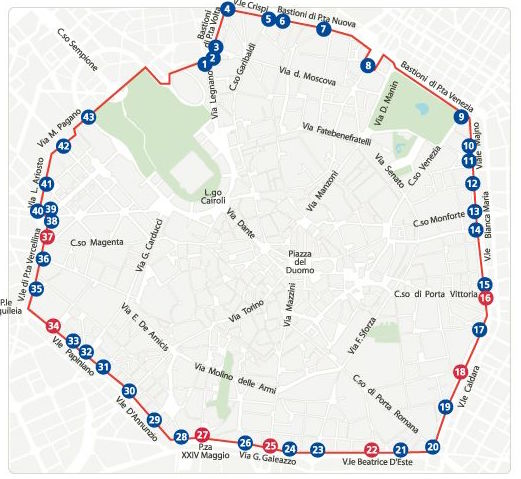
\includegraphics[width=.64\textwidth]{../img/milan-map.jpg}
	\caption{Milan Ecopass/Area C \citep{Rotaris2010}}
	\label{fig:milan-map}
\end{figure}

\begin{table}
\begin{center}
\begin{tabular}{|>{\centering}m{1.8cm}|>{\centering}m{1.8cm}|>{\centering}p{1.8cm}|}
\hline 
Emissions Class & Charge (\euro) \tabularnewline
\hline 
\hline 
1 & 0 \tabularnewline
\hline 
2 & 0 \tabularnewline
\hline 
3 & 2 \tabularnewline
\hline 
4 & 5 \tabularnewline
\hline 
5 & 10 \tabularnewline
\hline 
\end{tabular}
\par\end{center}
\caption{Ecopass prices. Lower classes are less polluting. Class I includes hybrid and electric cars. Class V low-efficiency diesel and buses. \citep{Rotaris2010} }\label{tab:milan-ecopass-prices}
\end{table}

\begin{table}

\begin{center}
\begin{tabular}{|>{\centering}m{2.2cm}|>{\centering}m{1.8cm}|}
\hline 
User Class & Charge (\euro)\tabularnewline
\hline 
\hline 
standard & 5\tabularnewline
\hline 
residents & 2\tabularnewline
\hline 
commercial & 3\tabularnewline
\hline 
\end{tabular}
\par\end{center}
\caption{Area C prices \citep{Milan2015}}\label{tab:milan-area-c-prices}
\end{table}

\subsection{Results}

During the Ecopass trial, congestion inside the cordon fell by 12.3\%, vehicle-kilometers traveled by 14.2\% and accidents by 20.6\% while bus speeds and private vehicle speeds rose, respectively, 7.8\% and 4\% \citep{Rotaris2010}. Using time-series data during the suspension in summer 2012, \citet{Gibson2015} estimate that the suspension raised entries to the charging zone during charging hours by 27,500 per day (14.5 percent), CO concentrations by 6 percent and PM10 concentrations by 17 percent.
